\documentclass{article}
\usepackage{listings}
\usepackage{graphicx} %插入图片的宏包
\usepackage{float} %设置图片浮动位置的宏包
\usepackage{ctex}
\title{第一次实验}
\author{田鸿龙}
\date{\today}
\begin{document}
\maketitle
\section{Hello OS}
\subsection{运行截图}
\begin{figure}[H]
    \centering
    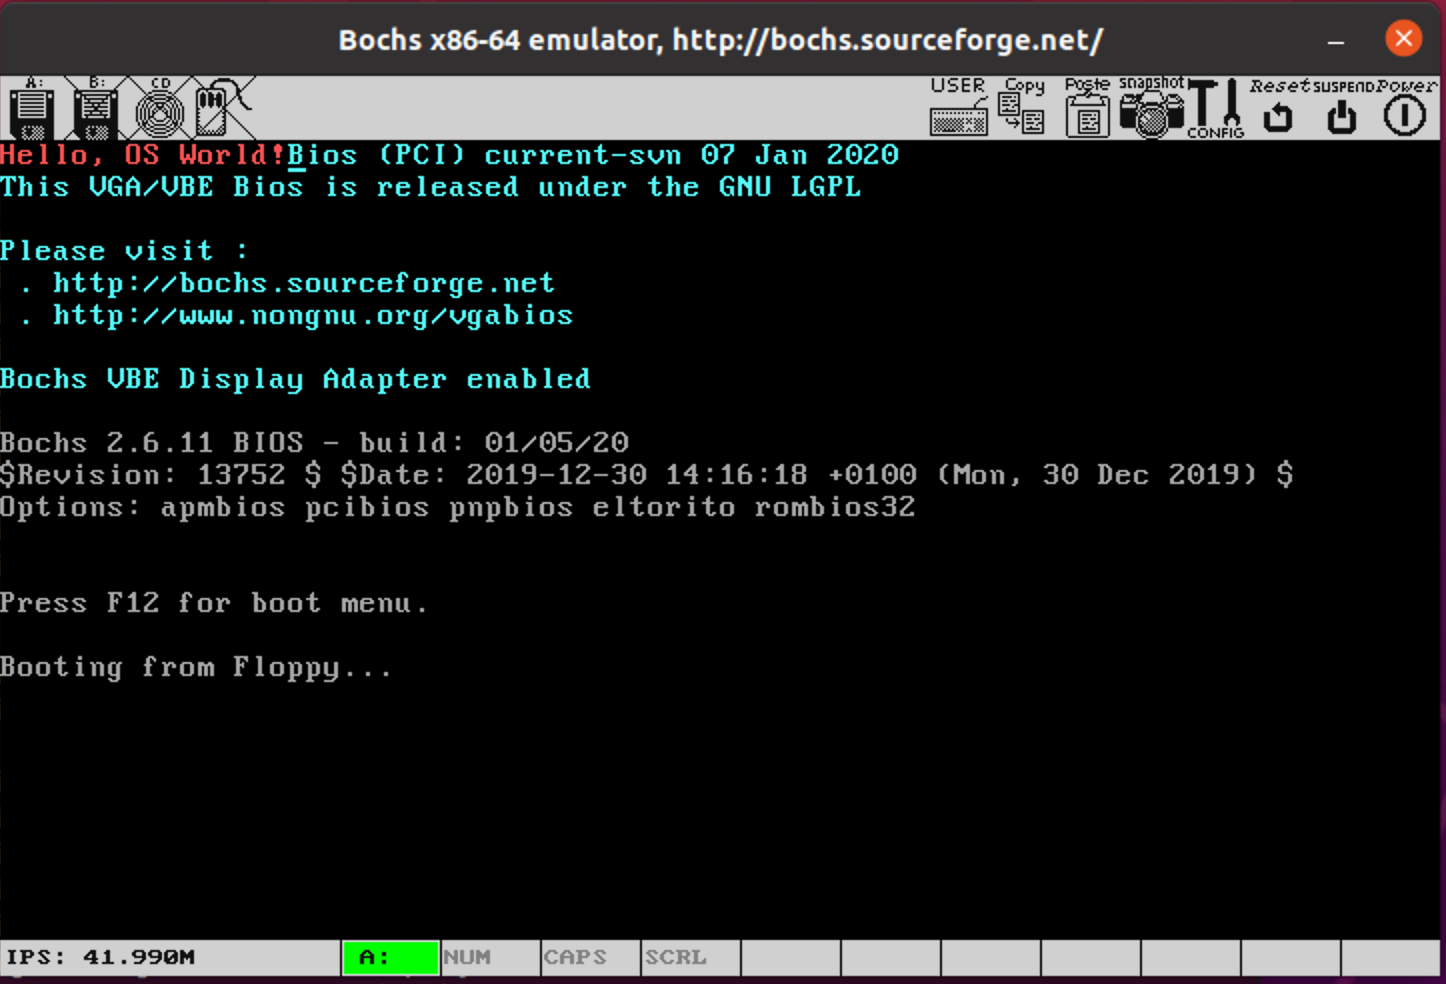
\includegraphics[width=0.7\textwidth]{bochs}
    \caption{bochs}
\end{figure}
\begin{figure}[H]
    \centering
    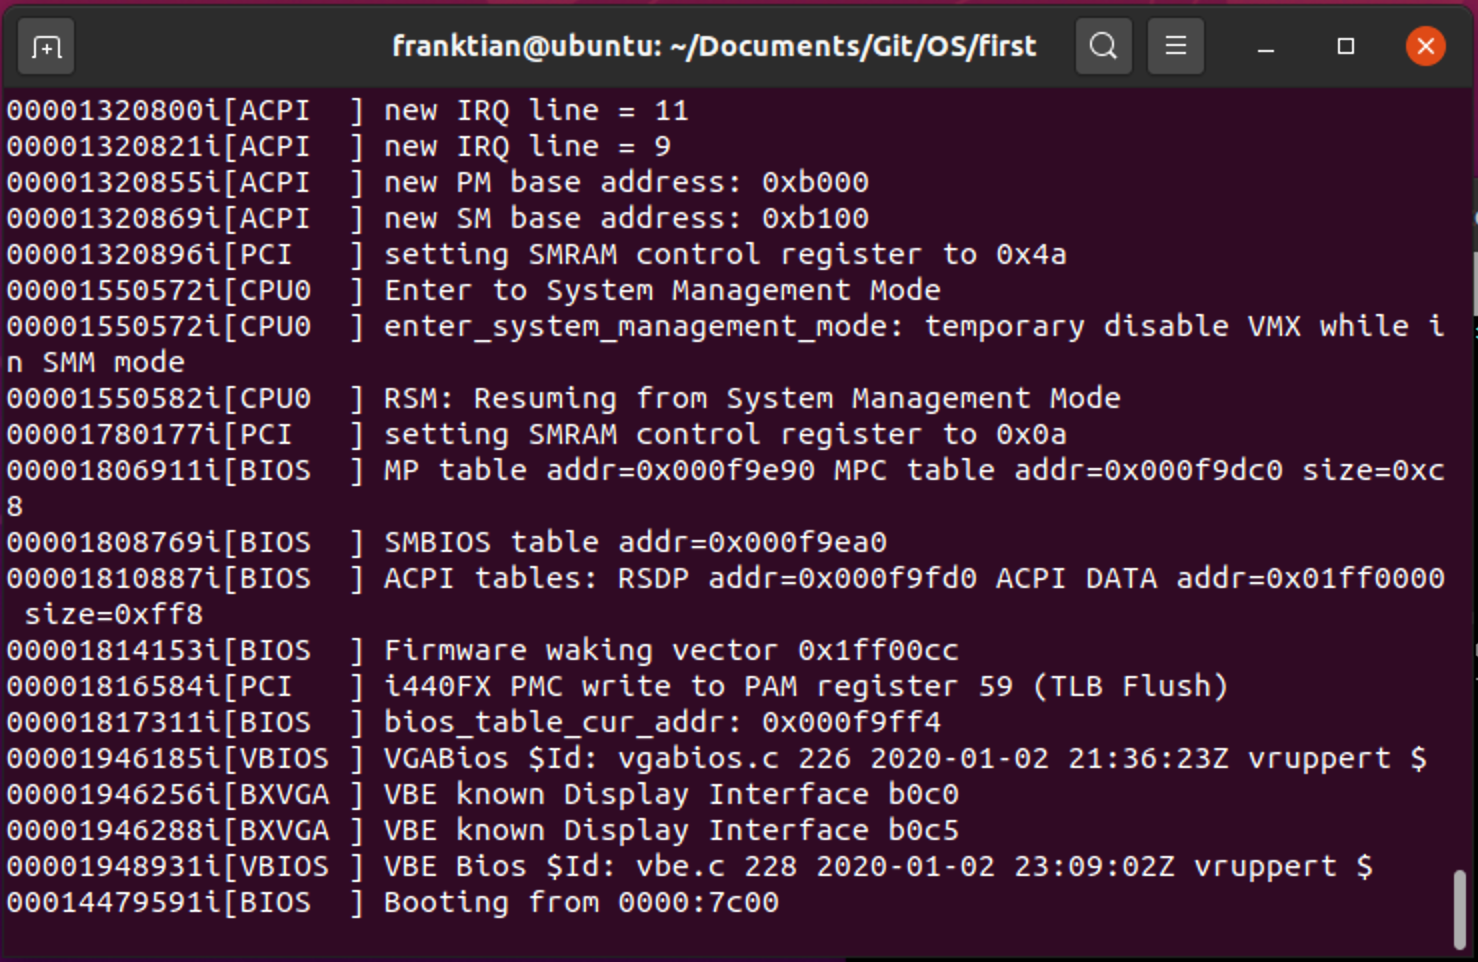
\includegraphics[width=0.7\textwidth]{terminal}
    \caption{terminal}
\end{figure}
\subsection{源代码}
\begin{lstlisting}
    org 07c00h
	mov ax, cs
	mov ds, ax
	mov es, ax
	call	DispStr
	jmp $
DispStr:
	mov ax, BootMessage
	mov bp, ax
	mov cx, 16
	mov ax, 01301h
	mov bx, 000ch
	mov dl, 0
	int 10h
	ret
BootMessage		db "Hello, OS World!"
times 510-($-$$)	db 0
dw 0xaa55
\end{lstlisting}[H]
\section{汇编语言实践}
\subsection{运行截图}
\begin{figure}
    \centering
    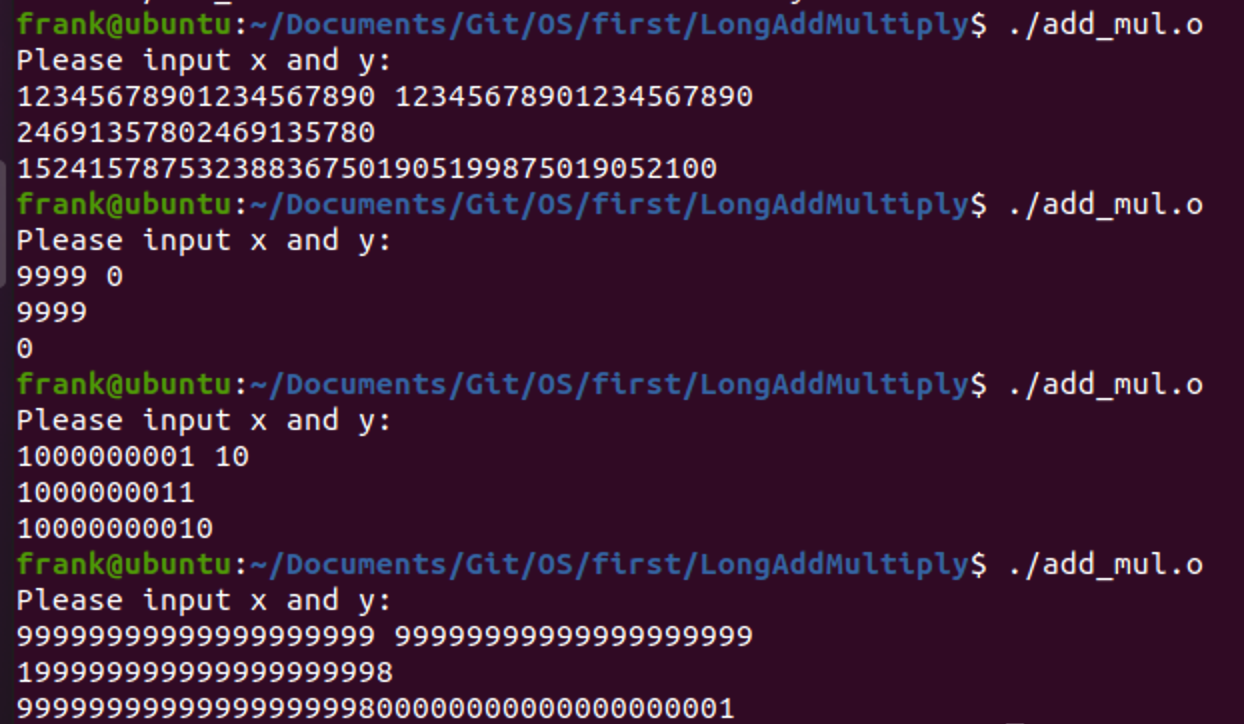
\includegraphics[width=0.7\textwidth]{add_mul_out}
    \caption{程序输出示例}
\end{figure}

\subsection{源代码}

在LongAddMultiply文件夹下的add\_mul.asm中。


\section{问题清单}
\subsection{请简述 80x86 系列的发展历史}
1978年6月,intel推出第一款16位微处理器8086,采用20位地址线。

1982年发布80286,主频提高至12MHz。

1985年发布80386,处理器变为32位,地址线扩展至32位。

1989年发布80486,1993年发布80586并命名为奔腾。
\subsection{说明小端和大端的区别,并说明 80x86 系列采用了哪种方式?}
在内存中,大端指的是从高字节开始,小端指的是从低字节开始。

80x86是小端。

\subsection{8086 有哪五类寄存器,请分别举例说明其作用?}
数据寄存器,指针寄存器,变址寄存器,控制寄存器,段寄存器。

\subsection{什么是寻址?立即寻址和直接寻址的区别是什么?}
寻址即找到操作数段地址。

立即寻址直接给出了操作数,事实上没有“寻址”。

直接寻址直接给出了地址,通过地址从内存中取数据。
\subsection{请举例说明寄存器间接寻址、寄存器相对寻址、基址加变址寻址、相对基址加变址寻址四种方式的区别}

\subsection{请分别简述 MOV 指令和 LEA 指令的用法和作用?}
lea是“load effective address”的缩写,简单的说,lea指令可以用来将一个内存地址直接赋给目的操作数,例如:lea eax,[ebx+8]就是将ebx+8这个值直接赋给eax,而不是把ebx+8处的内存地址里的数据赋给eax。

而mov指令则恰恰相反,例如:mov eax,[ebx+8]则是把内存地址为ebx+8处的数据赋给eax。

\subsection{请说出主程序与子程序之间至少三种参数传递方式}
通过寄存器传递参数

通过堆栈传递参数

通过变量传递参数
\subsection{如何处理输入和输出,代码中哪里体现出来?}
使用syscall,在elf64环境下,0代表读,1代表写。

\subsection{有哪些段寄存器}
CS代码段

DS数据段

SS堆栈段

ES附加段
\subsection{通过什么寄存器保存前一次的运算结果,在代码中哪里体现出来。}
通过内存保存。
\subsection{解释 boot.asm 文件中,org 0700h 的作用}

\subsection{boot.bin 应该放在软盘的哪一个扇区?为什么?}
第一个,ROM中段BIOS程序会扫描第一个扇区。
\subsection{loader 的作用有哪些?}
跳入保护模式。

启动内存分页。

从kernel.bin中读取内核,并放入内存,然后跳转到内核所 在的开始地址,运行内核。
\subsection{解释 NASM 语言中 [ ] 的作用}


\subsection{解释语句 times 510-(\$-\$\$) db 0,为什么是 510? \$ 和 \$\$ 分别表示什么?}
\$表示当前地址

\$\$表示当前段的地址

将第一个扇区的前510个字节填充满,上最后两个字节为0xaa55。
\subsection{解释配置文件 bochsrc 文件中各参数的含义}
\begin{lstlisting}
megs:32
display_library: sdl
floppya: 1_44=a.img, status=inserted 
boot: floppy
\end{lstlisting}
megs:32表示虚拟机内存大小为32MB。

display\_library表示bochs使用的GUI库,在Ubuntu下面是sdl2.

floppya表示虚拟机的外设,这里指向了一个软盘。

boot表示虚拟机启动方式,从软盘启动。

吴雨瑄


\end{document}
